\chapter{Gestión del proyecto}
\label{section-gestion-proyecto}

Como proceso de inicio se establecieron con la empresa los objetivos y herramientas de trabajo del proyecto (nombrados en secciones anteriores). Además, se propuso al responsable del proyecto en la empresa una planificación inicial para organizar el trabajo de forma que se cumplieran los objetivos dentro del tiempo establecido. \\

Respecto al proceso de ejecución y control del proyecto, al ser un proyecto realizado de forma remota, se realizan regularmente reuniones mediante Google Meet con el responsable en la empresa. Por otro lado, para controlar el tiempo invertido en el proyecto se diseña una plantilla en la que diariamente se anotan las horas invertidas y se describen notas acerca del estado del proyecto o las tareas realizadas. \\

Como plan de gestión de configuraciones se establece que la documentación del proyecto se realiza en castellano. La implementación del frontend se realiza completamente en inglés y la implementación del backend se realiza utilizando inglés y castellano principalmente para que la empresa comprenda con mayor facilidad los comentarios en el código. Se destaca que, en la implementación del frontend, se configura el proyecto para utilzar Prettier \cite{prettier} y ESLint \cite{eslint} para formatear, analizar y detectar problemas en el código mejorando así la calidad del este. Respecto al control y alojamiento del código, se utiliza Git y GitHub para el frontend y un repositorio de la empresa para el backend. \\


Respecto al plan de construcción y despliegue del software se establece con la empresa que es suficiente con realizar la implementación y comporbar el funcionamiento del sistema con la conexión de los terminales en local, ya que posteriormente será la empresa la que utilizará el código como considere. \\

La planificación del proyecto como se ha comentado anteriormente se hizo al inicio del proyecto. Se establecío que el cronograma del trabajo a realizar debía ser el siguiente:
\begin{enumerate}
    \item Puesta en contexto, arranque de sistema de configuraciones y aprendizaje de herramientas y tecnologías a utilizar.
    \item Desarrollo del software dividido en las siguientes tareas:
    \begin{itemize}
        \item Revisión de diseño y requisitos con la empresa.
        \item Implementación del mockup del frontend.
        \item Implementación del backend (nuevo servicio en Helpnex).
        \item Union del frontend y backend.
        \item Comprobar correcto funcionamiento del sistema.
    \end{itemize}
    \item Documentación del proyecto (habiendo tomado las notas necesarias durante todo el desarrollo).
\end{enumerate}

En el Diagrama de Gantt (Véase \hyperref[fig:gantt]{Figura 4.1}) se pueden ver las tareas realizadas y el momento y duración dentro del proyecto de estas. En la planificación inicial se dió un par de semanas de margen para finalizar la implementación por si surgía cualquier inconveniente. Gracias a esta previsión, el tiempo invertido durante las dos primeras semanas de abril con el problema de utilizar la tencología SignalR (mencionado en otras secciones) realizando en pruebas, búsqueda de soluciones y planteamiento de las distintas opciones de la arquitectura, no ha supuesto un problema a la hora de finalizar con éxito la implementación y entrega del proyecto. Se comnsidera que el resto de planificación inicial es similar a la que se puede ver en el diagrama y que ha sido comentada en los enumeración. \\

En la planificación inicial se tenía también como objetivo monitorizar tareas (otro tipo de alerta) en la aplicación web, pero durante el desarrollo la empresa expresó la decisión de que, en la aplicación que querían ver de prueba, finalmente solo se quería monitorizar alarmas y presencias. En el diagrama, parte del tiempo invertido en el backend incluye la implemenación de este objetivo. Por esta razón, se decide dejar cierta parte funcional de forma que se pueda ver un ejemplo de cómo poder seguir con esa implementación, de cara a en un futuro decidir monitorizar tareas, y se elimina aquello que no sea útil o intervenga en la funcionalidad de los otros objetivos.

%como se indica en la \hyperref[section-trabajo-futuro]{sección 5.3}

\begin{landscape}
    \begin{figure}[!ht]
        \centering
        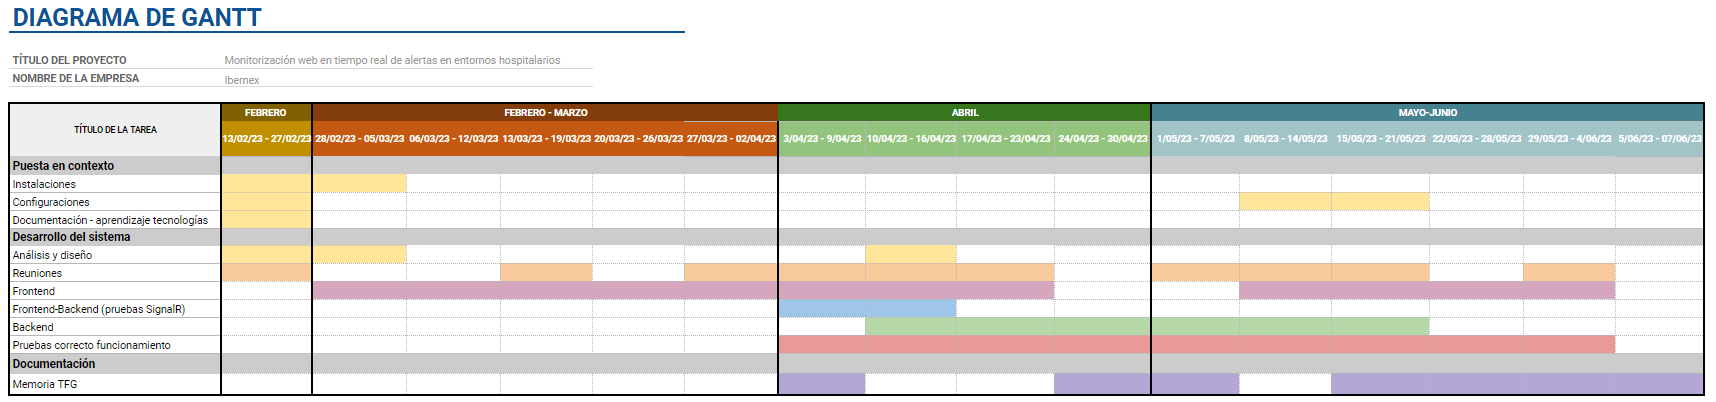
\includegraphics[width=25cm]{Imagenes/Diagrama-Gantt.PNG}
        \caption{Diagrama de Gantt}
        \label{fig:gantt}
    \end{figure}
\end{landscape}



